\let\negmedspace\undefined
\let\negthickspace\undefined

\documentclass[journal,12pt,onecolumn]{IEEEtran}
%\documentclass[journal,12pt,twocolumn]{IEEEtran}
%
\usepackage{setspace}
\usepackage{gensymb}
%\doublespacing
\singlespacing

%\usepackage{graphicx}
%\usepackage{amssymb}
%\usepackage{relsize}
\usepackage[cmex10]{amsmath}
%\usepackage{amsthm}
%\interdisplaylinepenalty=2500
%\savesymbol{iint}
%\usepackage{txfonts}
%\restoresymbol{TXF}{iint}
%\usepackage{wasysym}
\usepackage{amsthm}
\usepackage{mathrsfs}
\usepackage{txfonts}
\usepackage{stfloats}
\usepackage{cite}
\usepackage{cases}
\usepackage{subfig}
%\usepackage{xtab}
\usepackage{longtable}
\usepackage{multirow}
%\usepackage{algorithm}
%\usepackage{algpseudocode}
\usepackage{enumitem}
\usepackage{mathtools}
\usepackage{tikz}
\usepackage{circuitikz}
\usepackage{verbatim}
\usepackage{hyperref}
%\usepackage{stmaryrd}
\usepackage{tkz-euclide} % loads  TikZ and tkz-base
%\usetkzobj{all}
\usepackage{listings}
\usepackage{color}                                            %%
\usepackage{array}                                            %%
\usepackage{longtable}                                        %%
\usepackage{calc}                                             %%
\usepackage{multirow}                                         %%
\usepackage{hhline}                                           %%
\usepackage{ifthen}                                           %%
%optionally (for landscape tables embedded in another document): %%
\usepackage{lscape}     
\usepackage{multicol}
\usepackage{chngcntr}
\usepackage{iftex}
%\usepackage[latin9]{inputenc}
\usepackage{geometry}
\usepackage{bm}
%\geometry{verbose,tmargin=2cm,bmargin=3cm,lmargin=1.8cm,rmargin=1.5cm,headheight=2cm,headsep=2cm,footskip=3cm}
\usepackage{array}
\newcolumntype{L}[1]{>{\raggedright\let\newline\\\arraybackslash\hspace{0pt}}m{#1}}
\newcolumntype{C}[1]{>{\centering\let\newline\\\arraybackslash\hspace{0pt}}m{#1}}
\newcolumntype{R}[1]{>{\raggedleft\let\newline\\\arraybackslash\hspace{0pt}}m{#1}}

%\usepackage{graphicx}
%\usepackage{setspace}
%\usepackage{parskip}

\def \hsp {\hspace{3mm}}

\makeatletter

\providecommand{\tabularnewline}{\\}



\makeatother
\ifxetex
\usepackage[T1]{fontenc}
\usepackage{fontspec}
%\setmainfont[ Path = fonts/]{Sanskrit_2003.ttf}
\newfontfamily\nakulafont[Script=Devanagari,AutoFakeBold=2,Path = fonts/]{Nakula}
%\newfontfamily\liberationfont{Liberation Sans Narrow}
%\newfontfamily\liberationsansfont{Liberation Sans}
\fi
\usepackage{tikz}
\usepackage{xcolor}
%\usepackage{enumerate}

%\usepackage{wasysym}
%\newcounter{MYtempeqncnt}
\DeclareMathOperator*{\Res}{Res}
%\renewcommand{\baselinestretch}{2}
\renewcommand\thesection{\arabic{section}}
\renewcommand\thesubsection{\thesection.\arabic{subsection}}
\renewcommand\thesubsubsection{\thesubsection.\arabic{subsubsection}}

\renewcommand\thesectiondis{\arabic{section}}
\renewcommand\thesubsectiondis{\thesectiondis.\arabic{subsection}}
\renewcommand\thesubsubsectiondis{\thesubsectiondis.\arabic{subsubsection}}

% correct bad hyphenation here
\hyphenation{op-tical net-works semi-conduc-tor}
\def\inputGnumericTable{}                                 %%

\lstset{
	language=tex,
	frame=single, 
	breaklines=true
}

%\begin{document}
%


\newtheorem{theorem}{Theorem}[section]
\newtheorem{problem}{Problem}
\newtheorem{proposition}{Proposition}[section]
\newtheorem{lemma}{Lemma}[section]
\newtheorem{corollary}[theorem]{Corollary}
\newtheorem{example}{Example}[section]
\newtheorem{definition}[problem]{Definition}
%\newtheorem{thm}{Theorem}[section] 
%\newtheorem{defn}[thm]{Definition}
%\newtheorem{algorithm}{Algorithm}[section]
%\newtheorem{cor}{Corollary}
\newcommand{\BEQA}{\begin{eqnarray}}
	\newcommand{\EEQA}{\end{eqnarray}}
\newcommand{\define}{\stackrel{\triangle}{=}}
\bibliographystyle{IEEEtran}
%\bibliographystyle{ieeetr}
\providecommand{\mbf}{\mathbf}
\providecommand{\pr}[1]{\ensuremath{\Pr\left(#1\right)}}
\providecommand{\qfunc}[1]{\ensuremath{Q\left(#1\right)}}
\providecommand{\sbrak}[1]{\ensuremath{{}\left[#1\right]}}
\providecommand{\lsbrak}[1]{\ensuremath{{}\left[#1\right.}}
\providecommand{\rsbrak}[1]{\ensuremath{{}\left.#1\right]}}
\providecommand{\brak}[1]{\ensuremath{\left(#1\right)}}
\providecommand{\lbrak}[1]{\ensuremath{\left(#1\right.}}
\providecommand{\rbrak}[1]{\ensuremath{\left.#1\right)}}
\providecommand{\cbrak}[1]{\ensuremath{\left\{#1\right\}}}
\providecommand{\lcbrak}[1]{\ensuremath{\left\{#1\right.}}
\providecommand{\rcbrak}[1]{\ensuremath{\left.#1\right\}}}
\theoremstyle{remark}
\newtheorem{rem}{Remark}
\newcommand{\sgn}{\mathop{\mathrm{sgn}}}
\providecommand{\abs}[1]{\left\vert#1\right\vert}
\providecommand{\res}[1]{\Res\displaylimits_{#1}} 
\providecommand{\norm}[1]{\left\lVert#1\right\rVert}
%\providecommand{\norm}[1]{\lVert#1\rVert}
\providecommand{\mtx}[1]{\mathbf{#1}}
\providecommand{\mean}[1]{E\left[ #1 \right]}
\providecommand{\fourier}{\overset{\mathcal{F}}{ \rightleftharpoons}}
%\providecommand{\hilbert}{\overset{\mathcal{H}}{ \rightleftharpoons}}
%\providecommand{\system}{\overset{\mathcal{H}}{ \longleftrightarrow}}
\providecommand{\system}[1]{\overset{\mathcal{#1}}{ \longleftrightarrow}}
\providecommand{\gauss}[2]{\mathcal{N}\ensuremath{\left(#1,#2\right)}}
%
%\newcommand{\solution}[2]{\textbf{Solution:}{#1}}
\newcommand{\solution}{\noindent \textbf{Solution: }}
\newcommand{\cosec}{\,\text{cosec}\,}
\newcommand{\sinc}{\,\text{sinc}\,}
\newcommand{\rect}{\,\text{rect}\,}
\providecommand{\dec}[2]{\ensuremath{\overset{#1}{\underset{#2}{\gtrless}}}}
\newcommand{\myvec}[1]{\ensuremath{\begin{pmatrix}#1\end{pmatrix}}}
\newcommand{\mydet}[1]{\ensuremath{\begin{vmatrix}#1\end{vmatrix}}}
\newcommand*{\permcomb}[4][0mu]{{{}^{#3}\mkern#1#2_{#4}}}
\newcommand*{\perm}[1][-3mu]{\permcomb[#1]{P}}
\newcommand*{\comb}[1][-1mu]{\permcomb[#1]{C}}
%\numberwithin{equation}{section}
\numberwithin{equation}{section}
%\numberwithin{problem}{section}
%\numberwithin{definition}{section}
\makeatletter
\@addtoreset{figure}{problem}
\makeatother
%\let\StandardTheFigure\thefigure
\let\vec\mathbf
%\renewcommand{\thefigure}{\theproblem.\arabic{figure}}
\renewcommand{\thefigure}{\arabic{section}.\arabic{figure}}
%\setlist[enumerate,1]{before=\renewcommand\theequation{\theenumi.\arabic{equation}}
	%\counterwithin{equation}{enumi}
	%\renewcommand{\theequation}{\arabic{subsection}.\arabic{equation}}
\let\StandardTheFigure\thefigure
	\vspace{3cm}
	%\usepackage{babel}
	\begin{document}
		\title{DBSCAN}
		\author{ Mannem Charan AI21BTECH11019}
		 \maketitle
		\begin{abstract}
			This report consists of my basic understanding of one of the popular Ml methods "DBSCAN".
		\end{abstract}
		\section{DBSCAN}
		  DBSCAN is an unsupervised learning algorithm and used for clustering problems.Every clustering method follows the same approach i.e., it will try group the \textbf{similar} data points together as clusters.Although we have $k$-means clustering algorithm to do clustering , sometimes it fail to show the results that we need and DBSCAN can be used as a replacement for $k$-means.
		 \section{DBSCAN vs $k$-means}
		   To understand where $k$-means fails to do the job let us consider the dataset shown in fig $\ref{1}$,
		     \begin{figure}[ht!]
		      \centering
	              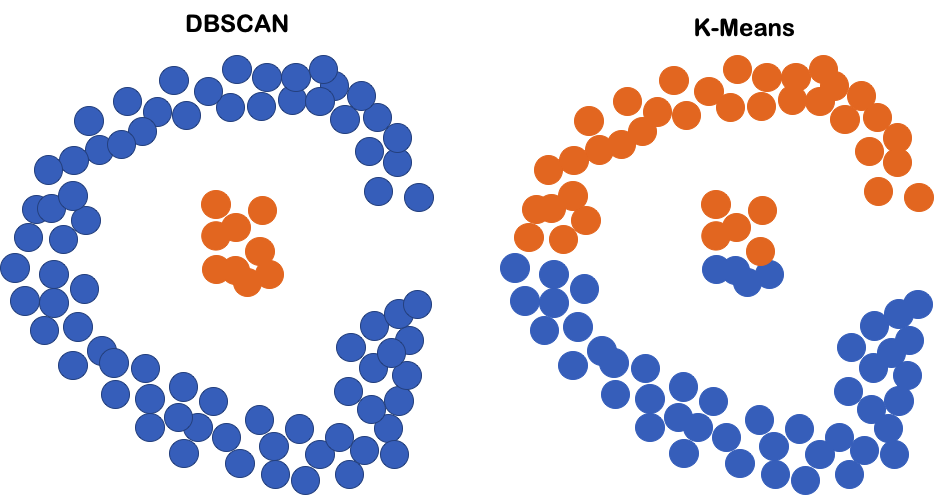
\includegraphics[width = 10cm]{1.png}
		      \caption{DBSCAN vs K-means}
		      \label{1}
		     \end{figure}
          The $k$-means algorithm which works on distance between the points identifies the clusters w.r.t the mean points so sometimes it may not be similar to how a human eye clusters the data.In $\ref{1}$, DBSCAN able to mimic how a human eye identifies the clusters.So for this type of data it is best to use DBSCAN.DBSCAN works based on the densities of the points.
	          \section{How DBSCAN works?}
		    DBSCAN is a density-based clustering algorithm and the clusters are made sequentially one after other.To understand that let us take some unclustered data as shown in fig $\ref{2}$.
		    \begin{figure}[ht!]
		     \centering
		     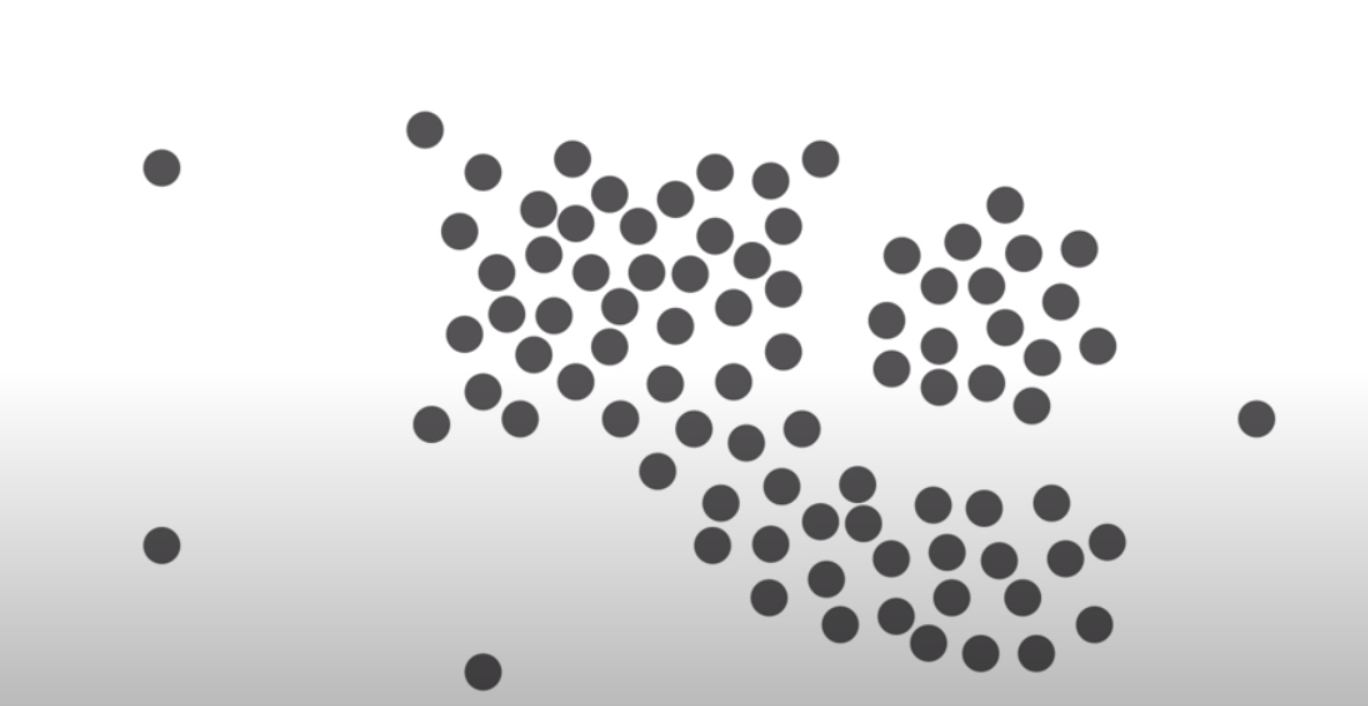
\includegraphics[width = 10cm]{raw_data.png}
		     \caption{unclustered data}
		     \label{2}
		    \end{figure}
	Now one thing that we can do is count the number of points close to each point. In DBSCAN,we will do it by taking a small circle around the data point and the data points which are inside/crossing this circle are considered to closer to the given data point.In this case the red point is close to 8 data points in fig $\ref{3}$
	      \begin{figure}[ht!]
		\centering
		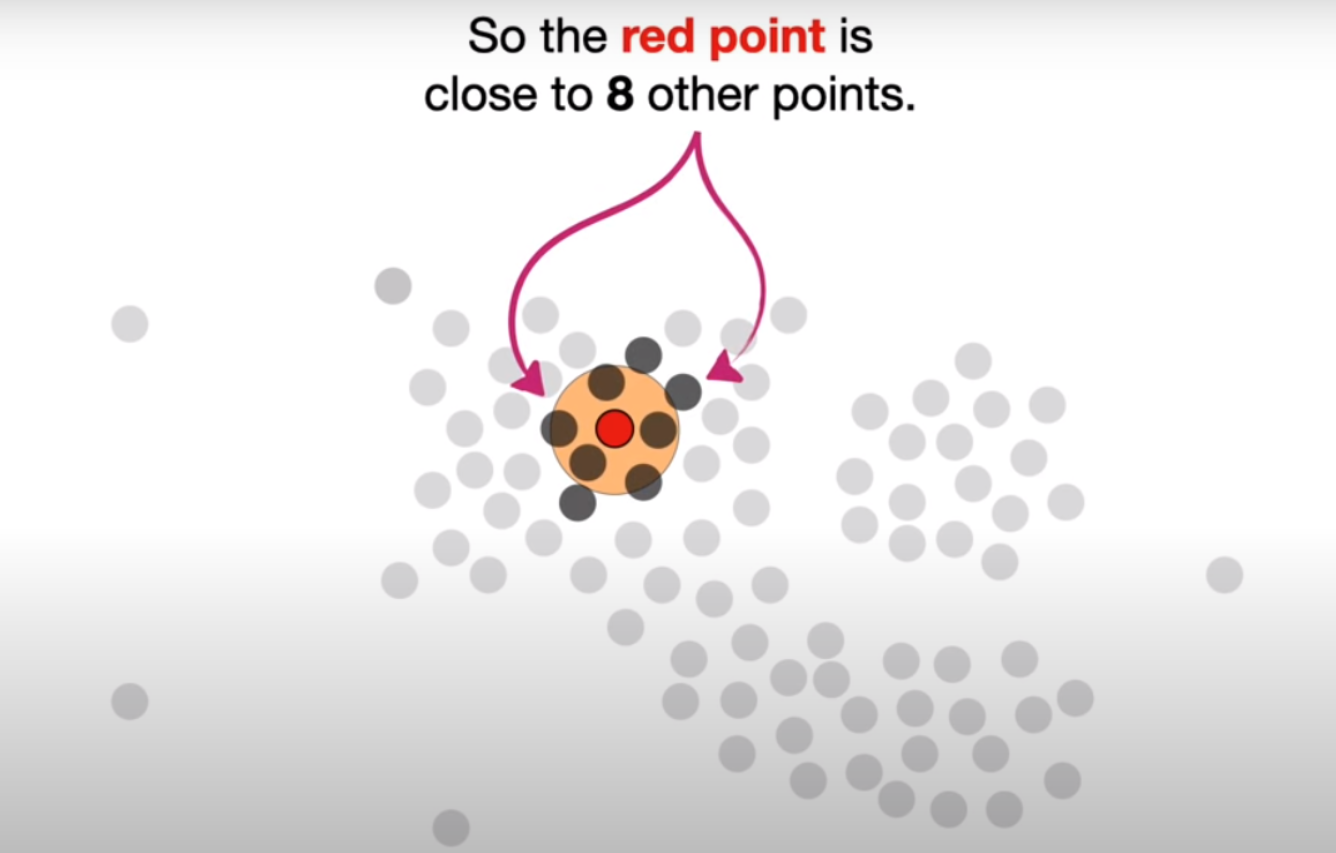
\includegraphics[width=10cm]{2.png}
		\caption{}
		\label{3}
	      \end{figure}
	 And the radius of circle used for finding the number of points closer to given data point is user defined known as "\textbf{eps}"$\brak{\epsilon}$. It is one of the tuneable parameters in DBSCAN. And like this we will see the neighbourhood of each point and count the no. of points \textbf{closer} to each point.\\
	 Then we define something called core point which has neighbouring points greater than certain threshold.This threshold is known as "\textbf{minPts}". This threshold decides whether a neighbourhood around data point is "dense" enough.This parameter is also user-defined and tuneable.Using this parameter, we will find all core points in the data.In this case we took threshold as 4 points and  the core points of the data are shown in fig $\ref{4}$,\\
	     \begin{figure}[ht!]
	      \centering
	      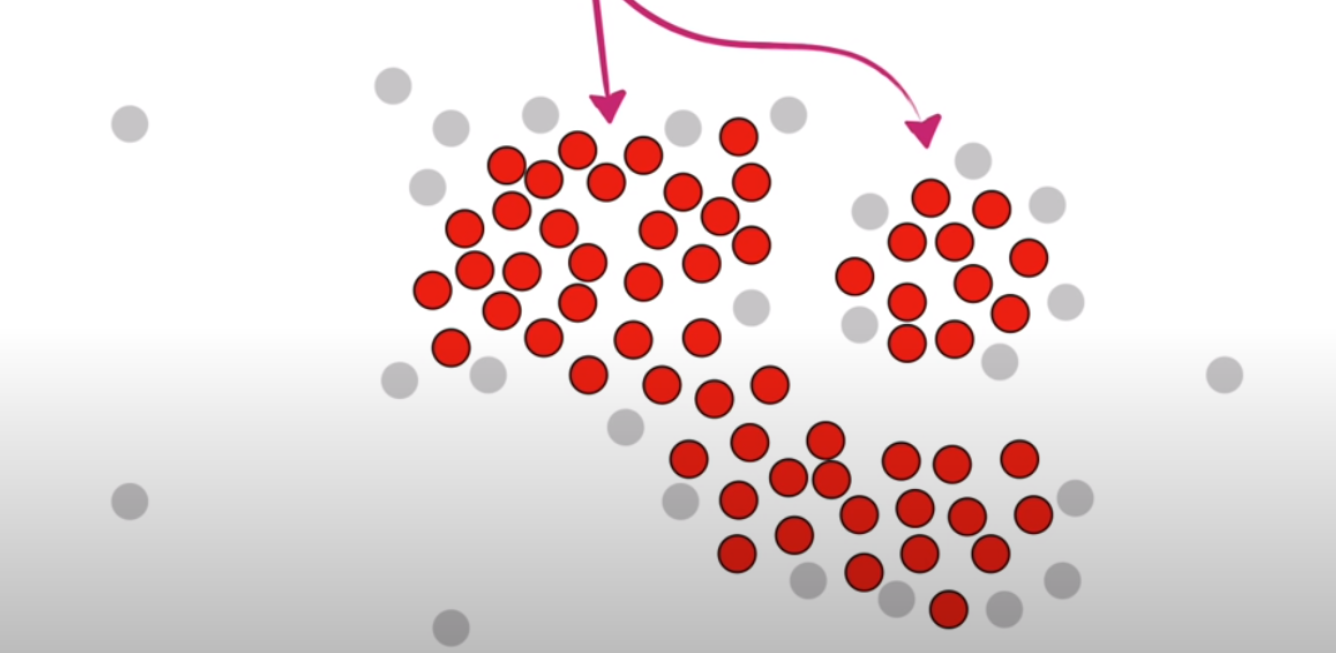
\includegraphics[width=10cm]{3.png}
	      \caption{Core points marked as red dots}
	      \label{4}
             \end{figure}
	   And remaining data points are non-core points.After that we randomly pick a core point and assign it to the first cluster.And then we will assign all the core points which are closer the given core point to the first cluster.Similarly we will add all core points closer to the points in the cluster and so on.Like that the cluster will grow eventually but at each step we are only adding the core points to the cluster $\brak{\text{atleat for now}}$ neglecting the non-core points.After we add all core points to the cluster we then add the non-core points which are \textbf{closer} to the points of cluster.Note that only core points are responsible for growing the cluster, non-core points are added to cluster depending on how close they are with core points.And like that we will identify the first cluster as shown in fig $\ref{5}$.
	   \begin{figure}[ht!]
            \centering
	    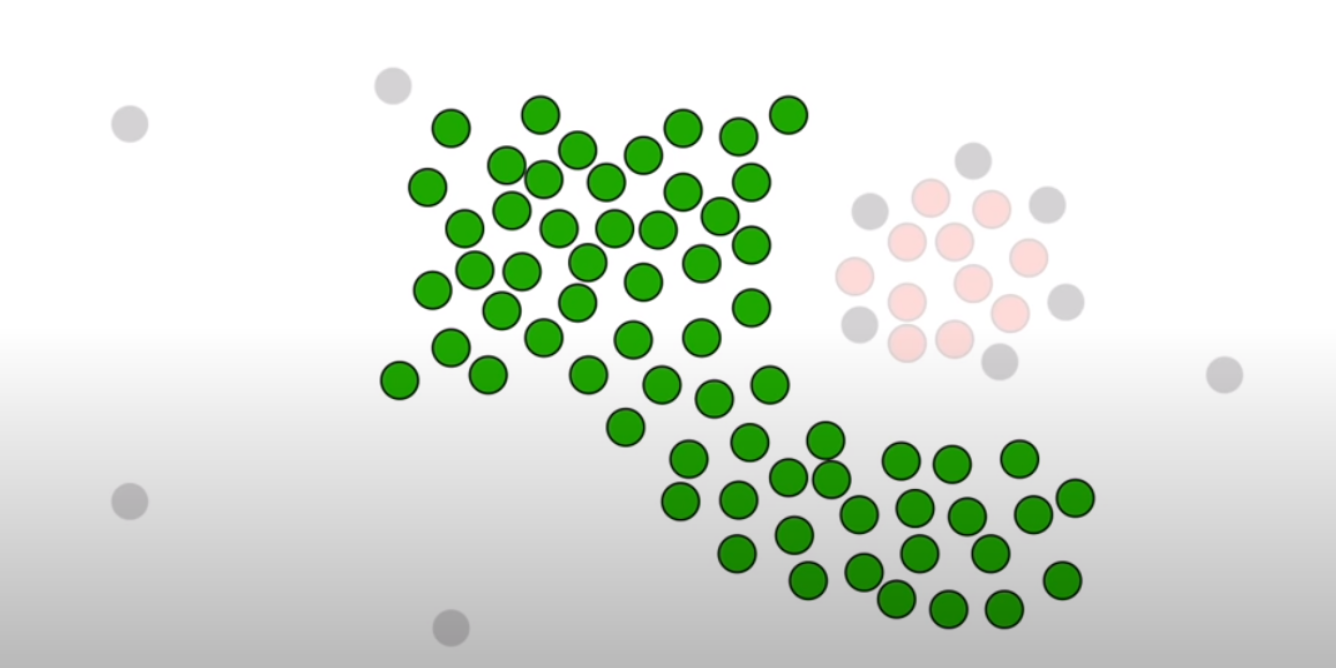
\includegraphics[width=10cm]{4.png}
	    \caption{First cluster}
	    \label{5}
	   \end{figure}
	Similarly you will form the second cluster by taking the core point that is not included in first cluster.Overall the data set after clustering look like fig $\ref{6}$,
	   \begin{figure}[ht!]
	    \centering
	    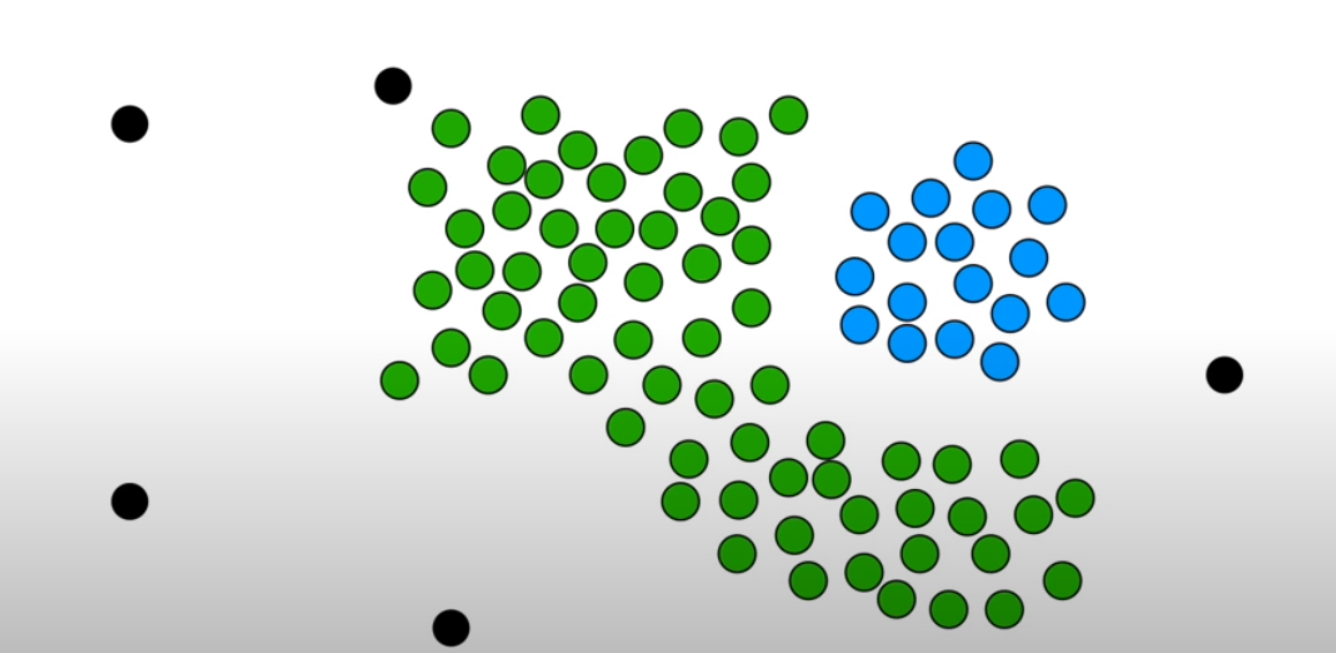
\includegraphics[width = 10cm]{5.png}
	    \caption{Clustered data}
	    \label{6}
	   \end{figure}
  It has been grouped into two clusters and with some outliers.And this ends the DBSCAN algorithm.
    \end{document}
